\section{Exemplos de conjuntos enumeráveis}

\begin{frame}[fragile]{Exemplos de conjuntos enumeráveis}

    \begin{enumerate}
        \item Os números naturais são enumeráveis: eles são enumerados pela função identidade
            $f(n) = n$

        \item A união dos números naturais com o zero também é enumerável: a função 
            $g:\mathbb{N}\to \mathbb{N}\cup \lbrace 0\rbrace$ tal que
            \[
                g(n) = n - 1
            \]
            enumera esta união

        \item O conjunto dos naturais pares é enumerado pela função total $h(n) = 2n$, ou
            pela parcial
            \[
                p(n) = \left\lbrace \begin{array}{ll}
                            n, & \mbox{se}\ n\ \mbox{é par} \\
                            \mbox{indefinida}, & \mbox{caso contrário}
                        \end{array}\right.
            \]
    \end{enumerate}

\end{frame}

\begin{frame}[fragile]{Exemplos de conjuntos enumeráveis}

    \begin{enumerate}
        \setcounter{enumi}{3}
        \item O conjunto vazio $\emptyset$ é enumerado pela a função $z(n) =$ indefinida,
            $\forall n\in \mathbb{N}$ 

        \item Qualquer conjunto finito $A$ é enumerável

        \item Os números inteiros $\mathbb{Z}$ são enumeráveis: uma listagem possível dos seus
        elementos é
        \[
            0, -1, 1, -2, 2, -3, 3, \ldots
        \]
        Uma função $f$ que gera tal enumeração é 
        \[
            f(n) = \left\lbrace \begin{array}{ll}
                        \frac{n - 1}{2}, & \mbox{se}\ n\ \mbox{é ímpar} \\
                        -\frac{n}{2}, & \mbox{caso contrário}
                    \end{array}\right.
        \]

    \end{enumerate}

\end{frame}

\begin{frame}[fragile]{Enumerabilidade dos números racionais}

    \begin{block}{Teorema}
        O conjunto dos números racionais positivos $\mathbb{Q}^+$ é enumerável.
    \end{block}

    \vspace{0.2in}

    Para demonstrar este importante resultado, observe que
    \[
        \mathbb{Q}^+ = \lbrace (a, b)\ |\ a, b\in \mathbb{N}\rbrace
    \]

    Assim, basta demostrar o seguinte lema:

    \begin{block}{Lema}
        O conjunto os pares ordenados de números naturais é enumerável.
    \end{block}

\end{frame}

\begin{frame}[fragile]{Demonstração por {\it zigue-zague} de Cantor} 

    \begin{figure}[h]
        \centering
        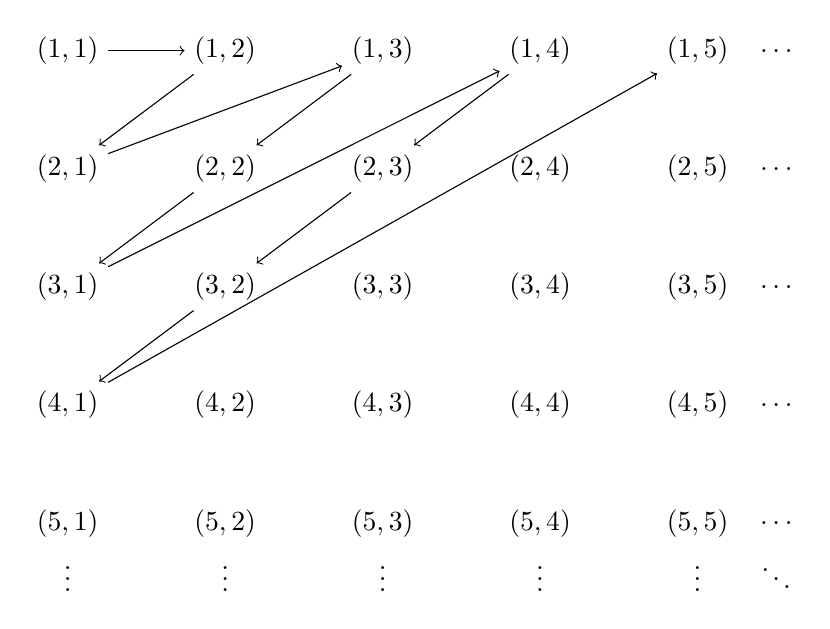
\begin{tikzpicture}
            \node (11) at (1, 9) { $(1, 1)$ };
            \node (12) at (3, 9) { $(1, 2)$ };
            \node (13) at (5, 9) { $(1, 3)$ };
            \node (14) at (7, 9) { $(1, 4)$ };
            \node (15) at (9, 9) { $(1, 5)$ };
            \node at (10, 9) { $\ldots$ };

            \node (21) at (1, 7.5) { $(2, 1)$ };
            \node (22) at (3, 7.5) { $(2, 2)$ };
            \node (23) at (5, 7.5) { $(2, 3)$ };
            \node (24) at (7, 7.5) { $(2, 4)$ };
            \node (25) at (9, 7.5) { $(2, 5)$ };
            \node at (10, 7.5) { $\ldots$ };

            \node (31) at (1, 6) { $(3, 1)$ };
            \node (32) at (3, 6) { $(3, 2)$ };
            \node (33) at (5, 6) { $(3, 3)$ };
            \node (34) at (7, 6) { $(3, 4)$ };
            \node (35) at (9, 6) { $(3, 5)$ };
            \node at (10, 6) { $\ldots$ };

            \node (41) at (1, 4.5) { $(4, 1)$ };
            \node (42) at (3, 4.5) { $(4, 2)$ };
            \node (43) at (5, 4.5) { $(4, 3)$ };
            \node (44) at (7, 4.5) { $(4, 4)$ };
            \node (45) at (9, 4.5) { $(4, 5)$ };
            \node at (10, 4.5) { $\ldots$ };


            \node (51) at (1, 3) { $(5, 1)$ };
            \node (52) at (3, 3) { $(5, 2)$ };
            \node (53) at (5, 3) { $(5, 3)$ };
            \node (54) at (7, 3) { $(5, 4)$ };
            \node (55) at (9, 3) { $(5, 5)$ }; 
            \node at (10, 3) { $\ldots$ };

            \node at (1, 2.4) { $\vdots$ };
            \node at (3, 2.4) { $\vdots$ };
            \node at (5, 2.4) { $\vdots$ };
            \node at (7, 2.4) { $\vdots$ };
            \node at (9, 2.4) { $\vdots$ };
            \node at (10, 2.4) { $\ddots$ };

            \draw[->] (11) edge (12);
            \draw[->] (12) edge (21);
            \draw[->] (21) edge (13);
            \draw[->] (13) edge (22);
            \draw[->] (22) edge (31);
            \draw[->] (31) edge (14);
            \draw[->] (14) edge (23);
            \draw[->] (23) edge (32);
            \draw[->] (32) edge (41);
            \draw[->] (41) edge (15);
        \end{tikzpicture}
    \end{figure}

\end{frame}

\begin{frame}[fragile]{Demonstração por {\it zigue-zague} de Cantor} 

    \begin{itemize}
        \item A função $G$ que enumera os pares é tal que 
        \[
            G(1) = (1, 1), G(2) = (1, 2), G(3) = (2, 1), G(4) = (1, 3), \ldots
        \]
        conforme padrão apresentado na figura anterior

        \item O padrão, de fato, é o seguinte: primeiro são enumerados todos os pares cujas
            coordenadas somam $2$ (a saber, apenas o par $(1, 1)$)

        \item Em seguida, são listados todos os pares cujas coordenadas somam $3$, ordenados
            pela primeira coordenada: $(1, 2), (2, 1)$

        \item Após estes são enumerados os pares que somam $4, 5, \ldots$, e assim por diante

        \item É possível, mas não necessário, descrever a função $G$ em termos de $n$
    \end{itemize}

\end{frame}

\begin{frame}[fragile]{Enumerabilidade das sequências finitas de inteiros positivos}

    \begin{block}{Proposição}
        O conjunto $\mathcal{S}$ de todas as sequências finitas de inteiros positivos é enumerável.
    \end{block}
\end{frame}

\begin{frame}[fragile]{Enumerabilidade das sequências finitas de inteiros positivos}
    \begin{block}{Demonstração}
        O Teorema Fundamental da Aritmética nos diz que qualquer inteiro $n\geq 2$ pode ser 
        escrito, de forma única, como
        \[
            n = p_1^{\alpha_1}p_2^{\alpha_2}\ldots p_k^{\alpha_k},
        \]
        onde os números $p_i$ são primos e os expoentes $\alpha_i$ são inteiros não-negativos.
        A função $f(s)$ recebe uma sequência finita de inteiros positivos 
        $s = \lbrace s_1, s_2, \ldots, s_N\rbrace$ e retorna o natural
        \[
            f(s) = 2^{s_1}3^{s_2}5^{s_3}\ldots p_N^{s_N},
        \]
        onde $p_N$ é o $N$-ésimo número primo. 
        Fazendo $f(e) = 1$, onde $e$ é a sequência vazia, a inversa da função $f$ pode ser usada
        para construir uma função parcial $G$ que enumera $\mathcal{S}$.
    \end{block}
    
\end{frame}

\begin{frame}[fragile]{Exemplos da enumeração de $\mathcal{S}$}

    \begin{enumerate}
        \item A sequência de três termos $s = \lbrace 1, 2, 3\rbrace$ é codificada pelo número
        $2250$ pela função $f$, pois
        \[
            f(s) = 2^13^25^3 = 2250
        \]

        \item A sequência $s$ tal que $f(s) = 30$ é $s = \lbrace 1, 1, 1\rbrace$, pois
        \[
            30 = 2^13^15^1
        \]

        \item As cinco primeiras sequências da enumeração são
        \[
            e, \lbrace 1\rbrace, \lbrace 2\rbrace, \lbrace 1, 1\rbrace, \lbrace 3\rbrace
        \]

        \item Veja, na listagem acima, que a função $G(n) = f^{-1}(n)$ não está definida para
            todos os $n$ naturais
    \end{enumerate}

\end{frame}

\begin{frame}[fragile]{Enumerabilidade das cadeias finitas de alfabetos enumeráveis}

    \begin{block}{Proposição}
        Seja $\mathcal{A}$ um alfabeto enumerável. O conjunto $\mathcal{C}$ de todas as cadeias 
        finitas de símbolos de $\mathcal{A}$ é enumerável.
    \end{block}

    \begin{block}{Demonstração}
        Como $\mathcal{A}$ é enumerável, seus elementos podem ser dispostos em ordem:
        \[
            \mathcal{A} = \lbrace a_1, a_2, a_3, \ldots\rbrace
        \]

        Assim, qualquer cadeia finita $c = \lbrace a_{i_1}a_{i_2}\ldots a_{i_N}\rbrace\in\mathcal{C}$ 
        corresponde uma sequência finita de inteiros positivos
        \[
            s = \lbrace i_1, i_2, \ldots, i_N\rbrace
        \]
        Como $\mathcal{S}$ é enumerável, $\mathcal{C}$ também é enumerável.
    \end{block}


\end{frame}
% Adicionar a enumerabilidade das sequências de números inteiros e das cadeias finitas de alfabetos enumeráveis
